\documentclass{article}
\usepackage{amsmath,amsthm,graphicx,siunitx}
\newtheorem{definition}{Definition}
\newcommand{\ket}[1]{\left|#1\right\rangle}

\title{Decoherence of a driven qubit}
\author{Ada Lovelace \and Erwin Example}

\begin{document}
\maketitle

\begin{abstract}
We model a resonantly driven two-level system coupled to a Markovian bath and show how the
Rabi oscillations of Figure~\ref{fig:rabi} decay. The page you are reading is a plain
LaTeX file, compiled by mystmd and rendered by Astro; numbering, references and citations
are resolved across this article and its Markdown supplement.
\end{abstract}

\section{Introduction}\label{sec:intro}

The unitary dynamics of a closed system follows the Schr\"odinger equation~\cite{schrodinger1926}.
Open systems require a master equation, introduced in Section~\ref{sec:model};
for background see \citet{nielsen2010}.

\section{Model}\label{sec:model}

\begin{definition}\label{def:lindblad}
A Lindblad master equation has the form
\begin{equation}
  \dot\rho = -\frac{i}{\hbar}[H,\rho] + \gamma\left(L\rho L^\dagger - \tfrac12\{L^\dagger L,\rho\}\right).
  \label{eq:lindblad}
\end{equation}
\end{definition}

For a qubit driven at frequency $\Omega$ with decay rate $\gamma$ we use
\begin{align}
  H &= \frac{\hbar\Omega}{2}\,\sigma_x, &
  L &= \sigma_- . \label{eq:hamiltonian}
\end{align}
Equation~\eqref{eq:lindblad} with the operators of Eq.~\eqref{eq:hamiltonian} is of the form
proven general by \citet{lindblad1976}.

\section{Results}\label{sec:results}

\begin{figure}
  \centering
  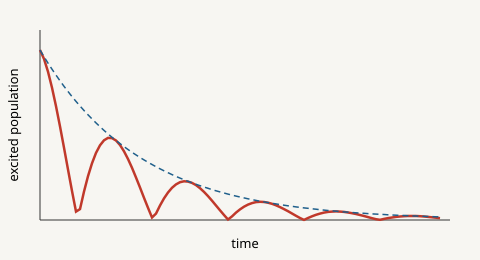
\includegraphics[width=0.8\textwidth]{figures/rabi.svg}
  \caption{Excited-state population (solid) and its envelope $e^{-\gamma t/2}$ (dashed).}
  \label{fig:rabi}
\end{figure}

\begin{table}
  \centering
  \caption{Parameters of the simulation.}
  \label{tab:params}
  \begin{tabular}{lll}
    \hline
    Symbol & Meaning & Value \\
    \hline
    $\Omega$ & Rabi frequency & \SI{10}{\mega\hertz} \\
    $\gamma$ & decay rate & \SI{0.5}{\mega\hertz} \\
    \hline
  \end{tabular}
\end{table}

With the parameters of Table~\ref{tab:params}, the population in Figure~\ref{fig:rabi}
decays as predicted by Definition~\ref{def:lindblad}. The trajectory on the Bloch sphere is
shown in Figure~\ref{fig-s-bloch} of the supplement, where the derivation of
Eq.~\eqref{eq-s-envelope} is given.

\section{Conclusion}

Section~\ref{sec:results} confirms the expected envelope.\footnote{All numbers on this page are generated by MyST.}

\end{document}
